\documentclass[a4paper,12pt]{article}
\usepackage[utf8]{inputenc}
\usepackage{amsmath}
\usepackage{biblatex}
\usepackage{color}
\usepackage{dirtree}
\usepackage{enumitem}
\usepackage{fancyhdr}
\usepackage{graphicx}
\usepackage{hyperref}
\usepackage{listings}
\usepackage{parallel}
\usepackage{pgf-umlsd}
\usepackage{subcaption}
\usepackage{tikz}
\usepackage{wrapfig}

\graphicspath{ {./img/} }
\usetikzlibrary{calc}
\usetikzlibrary{positioning}
\usetikzlibrary{shadows}
\usetikzlibrary{shapes.multipart}

\definecolor{dkgreen}{rgb}{0,0.6,0}
\definecolor{gray}{rgb}{0.5,0.5,0.5}
\definecolor{mauve}{rgb}{0.58,0,0.82}

\lstset{frame=tb,
	language=Java,
	aboveskip=3mm,
	belowskip=3mm,
	showstringspaces=false,
	columns=flexible,
	basicstyle={\small\ttfamily},
	numbers=none,
	numberstyle=\tiny\color{gray},
	keywordstyle=\color{blue},
	commentstyle=\color{dkgreen},
	stringstyle=\color{mauve},
	breaklines=true,
	breakatwhitespace=true,
	tabsize=3,
}

\addbibresource{documentation.bib}


\title{An Evaluation of the current State of web server development in Rust and Java
\footnote{This document references v0.5.0 of the GitHub Repository}}
\author{Marc Matija}
\date{\today}

\lhead{Marc Matija}
\rhead{\today}
\cfoot{\thepage}
\renewcommand{\headrulewidth}{0.4pt}
\renewcommand{\footrulewidth}{0.4pt}

\pagestyle{fancy}

\begin{document}
	\maketitle
	\vspace{2cm}
	\begin{abstract}
		This paper aims to evaluate the current state of web server development in Rust and Java. 
		In doing so, it will cover the basics of web server development in both languages, the tools and libraries 
		available, and the advantages and disadvantages of using each language for web server development. 
		Furthermore it will include a comparison of the two languages in terms of performance, ease of 
		use, and other factors that are important for web server development. 
	\end{abstract}
	
	\newpage
	\tableofcontents
	\newpage
	
	\section{Introduction}
	\label{sec:introduction}
	Web server development is an important aspect of modern software development as they are 
	used to host websites, web applications, and other online services.
	One of the most popular languages for this is Java and the Spring framework.
	Java is a mature and widely used programming language that is known for its performance, scalability, and reliability.
	However, in recent years, Rust has emerged as a promising alternative to Java for web server development as seen at Discord 
	\cite{Discord}, Cloudflare\cite{Cloudflare_Pingora}, and other companies. 
	Rust is in stark contrast to Java, is a systems programming language that is designed for performance, safety, and concurrency.
	This paper aims to evaluate the current state of web server development in Rust and Java, and to provide an overview of 
	the tools, libraries, and best practices for web server development in both languages.
	
	\subsection{An Overview of Spring Boot}
	\label{subsec:spring_boot}
	Spring Boot is a popular Java framework for building web applications and microservices used by companies like 
	Deutsche Bahn\cite{DB_Job_Description}, Udemy \cite{Techstack_Udemy} and many others\cite{Spring_Boot_stackshare}.
	Built on top of the Spring framework, Spring Boot provides a set of tools and libraries that make it easy to build
	web applications and microservices in Java. It finds wide adoption in the industry due to its ease of use, maintanability 
	and scalability, aswell as the vast amount of libraries and tools available for it.

	\subsection{An Overview of Actix Web}
	\label{subsec:actix_web}
	Actix is a Rust framework for building backend services in rust and the one currently one of the most actively developed framworks,
	within the Rust ecosystem. It provides provides a very similar feature set to Spring Boot making it a suitable candidate for comparison.

	\newpage
	\subsection{Other Used Technologies}
	\label{subsec:used_technologies}
	In addition to the frameworks mentioned above, I will use the following technologies to build the web server:
	\begin{itemize}
		\item \href{https://www.jetbrains.com/de-de/rust/}{RustRover} An IDE by Jetbrains that provides support for Rust development.
		\item \href{https://www.jetbrains.com/de-de/idea/}{IntelliJ IDEA Ultimate} An IDE by Jetbrains that provides support for Java development.
		\item \href{https://code.visualstudio.com/}{VS Code} A Text editor by microsoft used in this project for writing the LaTeX document.
		\item \href{https://www.postgresql.org/}{PostgreSQL} A popular open-source relational database management system that is widely used in the industry.
		\item \href{https://www.docker.com/}{Docker} A platform for building, shipping, and running applications in containers.
		\item \href{https://docs.docker.com/compose/}{Compose} A tool for defining and running multi-container Docker applications.
		\item \href{https://jwt.io/}{JWT} A standard for creating JSON-based access tokens that are used for authentication and authorization.
		\item \href{https://swagger.io/}{Swagger}  A tool for designing, building, and documenting APIs.
		\item \href{https://junit.org/junit5/}{JUnit} A popular testing framework for Java.
		\item \href{https://www.postman.com/}{Postman} A tool for testing APIs.
		\item \href{https://k6.io/}{K6} A tool for load testing web applications.
		\item \href{https://dbeaver.io/}{DBeaver} A database management tool.
		\item \href{https://chromewebstore.google.com/detail/talend-api-tester-free-ed/aejoelaoggembcahagimdiliamlcdmfm}{Talend API Tester} A tool for testing APIs.
	\end{itemize}

	\newpage
	\section{Specifications for the web server}
	\label{sec:example_project}
	In order to evaluate the current state of web server development in Rust and Java, I will build a simple web server in 
	both languages using the previously mentioned frameworks. The web server will feature a REST api that allows users to 
	create channels, add messages to channels, and retrieve messages from said channels. In addition, the web server will 
	feature a websocket endpoint that allows users to subscribe to channels and receive messages in real-time. Authentication 
	will be handled using JWT tokens and a profile endpoint to authenticate users and retrieve their information.

	\subsection{REST API}
	\label{subsec:rest_api}
	The REST API will feature the following endpoints:

	Channel endpoints:
	\begin{itemize}
		\item \textbf{Create Channel} \- POST /api/v1/channels \\
		Creates a new channel with the given name.
		\item \textbf{Get Channel} \- GET /api/v1/channels/\{id\} \\
		Retrieves the channel with the given id.
		\item \textbf{Get All Channels} \- GET /api/v1/channels \\
		Retrieves all channels.
		\item \textbf{Change Channel} \- PUT /api/v1/channels/\{id\} \\
		Changes the name of the channel with the given id.
		\item \textbf{Delete Channel} \- DELETE /api/v1/channels/\{id\} \\
		Deletes the channel with the given id.
	\end{itemize}

	Message endpoints:
	\begin{itemize}
		\item \textbf{Add Message} \texttt{ POST /api/v1/channels/\{id\}/messages } \\
		Adds a new message to the channel with the given id.
		\item \textbf{Get Message} \texttt{ GET /api/v1/channels/\{id\}/messages/\{id\} } \\
		Retrieves the message with the given id from the channel with the given id.
		\item \textbf{Get All Messages} \texttt{ GET /api/v1/channels/\{id\}/messages } \\
		Retrieves all messages from the channel with the given id.
		\item \textbf{Change Message} \texttt{ PUT /api/v1/channels/\{id\}/messages/\{id\} } \\
		Changes the content of the message with the given id from the channel with the given id.
		\item \textbf{Delete Message} \texttt{ DELETE /api/v1/channels/\{id\}/messages/\{id\}}
		Deletes the message with the given id from the channel with the given id.
	\end{itemize}

	% Authentication endpoints:
	% \begin{itemize}
	% 	\item \textbf{Sign up} \texttt{ POST /api/v1/auth/signup } \\
	% 	Registers a new user with the given username and password.
	% 	\item \textbf{Sign in} \texttt{ POST /api/v1/auth/signin } \\
	% 	Logs in the user with the given username and password.
	% 	\item \textbf{Sign out} \texttt{ POST /api/v1/auth/signout } \\
	% 	Logs out the currently logged in user.
	% \end{itemize}

	% Profile endpoints:
	% \begin{itemize}
	% 	\item \textbf{Get Profile} \texttt{ GET /api/v1/profile } \\
	% 	Retrieves the profile of the currently logged in user.
	% 	\item \textbf{Change Profile} \texttt{ PUT /api/v1/profile } \\
	% 	Changes the profile of the currently logged in user.
	% 	\item \textbf{Delete Profile} \texttt{ DELETE /api/v1/profile } \\
	% 	Deletes the profile of the currently logged in user.
	% \end{itemize}

	% \subsection{Websocket API}
	% \label{subsec:websocket_api}
	% In order to allow users to recieve messages in real-time, the web server will feature a websocket endpoint that 
	% allows users to subscribe to channels and receive updates when new messages are added to the channel. Users will
	% automatically be subscribed to Channels they are a part of. When establishing a connection to a websocket endpoint,
	% they will need to provide a valid JWT token in order to authenticate themselves.
	% \begin{itemize}
	% 	\item \textbf{Subscribe} \- \texttt{ws://localhost:8080/api/v1/ws} \\
	% 	Subscribes the user to the websocket endpoint and allows them to receive updates when new messages are added
	% 	to the channels they are a member of.
	% \end{itemize}
% 
	% \begin{wrapfigure}{L}{0.5\textwidth}
	% 	\begin{center}
	% 		\begin{sequencediagram}
	% 			\renewcommand\unitfactor{0.6}
	% 			\newthread{c}{Client}
	% 			\newinst[1]{s}{Web Server}
	% 			\begin{call}{c}{open()}{s}{}
	% 				\begin{call}{c}{auth()}{s}{}
	% 					\begin{call}{s}{verify()}{s}{}
	% 					\end{call}
	% 				\end{call}
	% 				\begin{sdblock}{New Message}{}
	% 					\begin{messcall}{s}{send()}{c}
	% 					\end{messcall}
	% 				\end{sdblock}
	% 				\begin{messcall}{c}{close()}{s}{}
	% 				\end{messcall}
	% 			\end{call}
	% 		\end{sequencediagram}
	% 	\end{center}
	% 	\caption[Message flow in a websocket connection]{Message flow in a websocket connection}
	% \end{wrapfigure}
	% 
	% In a websocket connection request, the headers of the HTTP request cannot be modified, the server will have to first 
	% accept the connection, then wait for the client to send a JWT token. The server will then verify the token and if it is 
	% valid, the client will be subscribed able to receive all messages from the channels they are a part of. Recieved 
	% messages will take the same format as the messages in the REST API.
	% \clearpage

	\newpage
	\subsection{Database Schema}
	\label{subsec:database_schema}
	The Implementations in both languages will feature the same PostgreSQL database, thus the database schema will 
	be the same for both implementations.
	\begin{figure}[h]
		\centering
		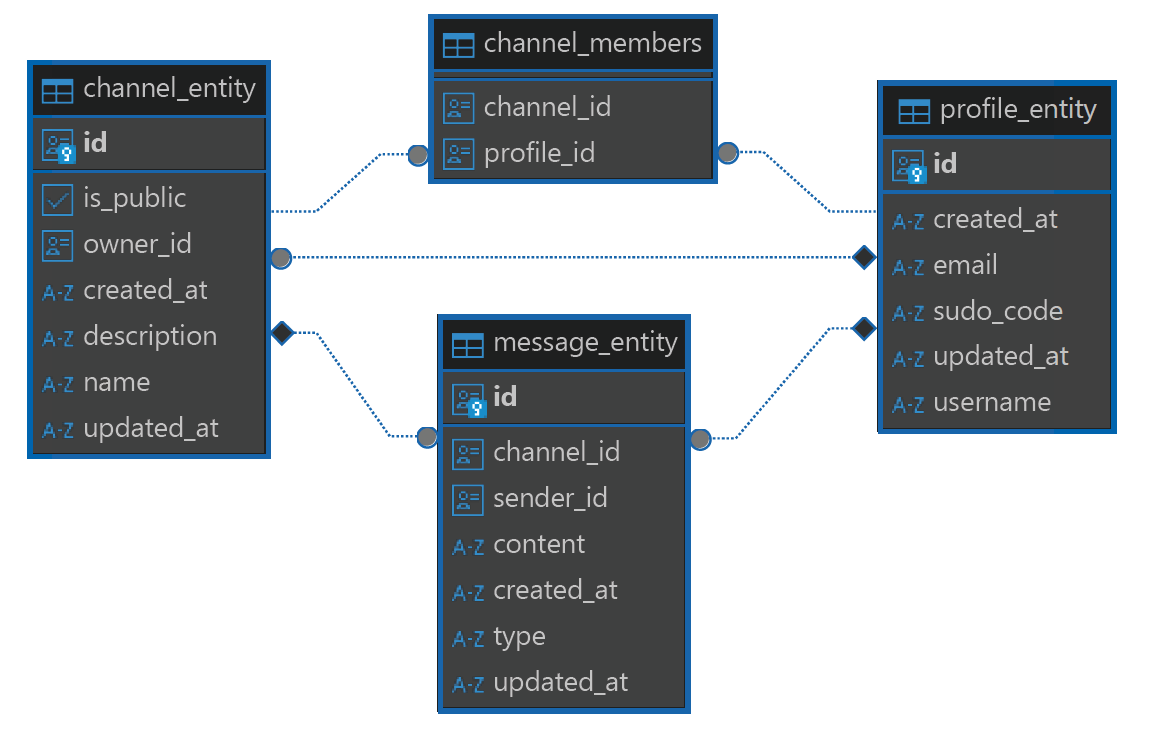
\includegraphics[width=\textwidth]{dbeaver_database_representation.png}
		\caption{Database schema in DBeaver}
		\label{fig:dbeaver_database_representation}
	\end{figure}

	It features a table for users, a table for channels, and a table for messages. The users table stores the username, email
	while the channels table stores the id of whoever created it, making him the \textbf{owner} of the channel. The messages table
	stores the content of the message, the id of the user who sent it, and the id of the channel it was sent to. All Tables also
	include coloumns for the creation and last update time of the row.

	\subsection*{A note about creation}
	A worthy note about the creation of this database schema is that it was not created by hand. For both Rust and Java I took
	the help of ORMs (Object Relational Mapper) which automatically map structures from each language into SQL statements. Spring
	JPA, the ORM used in the Spring-Boot implementation, has the ability to automatically create relations between entities by using
	anotations.
	\begin{lstlisting}
@Entity
@Table(name = "channel_entity")
public class ChannelEntity {
	/* ... */
	@ManyToMany
	@JoinTable(
			name = "channel_members",
			joinColumns = @JoinColumn(name = "channel_id"),
			inverseJoinColumns = @JoinColumn(name = "profile_id")
	)
	private List<ProfileEntity> members;
	/* ... */
}
	\end{lstlisting}
	The \textbf{@ManyToMany} annotation denotes a traditional Many to Many relationship in a relational database, allowing me to
	let JPA do the heavy lifting of creating all necesarry foreign keys and required Tables using the \textbf{@JoinTable} annotation.
	Further information about the workings of JPA can be found in the \hyperref[sec:java_implementation]{Java Implementation section}.

	\subsection{Authentication}
	\label{subsec:authentication}
	Authentication will be handled using JWT tokens. When a client signs up or signs in, they will receive a JWT token that
	they can use to authenticate themselves when making requests to the web server. The JWT token will be sent in the 
	Authorization header of the HTTP request as a Bearer token. Both Server implementations will have to verify the token 
	before sending new messages to the client.

	\section{Implementation in Java}
	\label{sec:java_implementation}
	\subsection{Project Structure}
	\label{subsec:project_structure_java}
	\begin{minipage}{0.4\textwidth}
		\dirtree{%
		.1 backendspringboot.
		.2 configuration.
		.2 controller.
		.2 data.
		.3 dto.
		.3 entities.
		.3 Mapper.
		.3 models.
		.3 repositories.
		.2 services.
	}%
	\clearpage
	\end{minipage}%
	\begin{minipage}{0.6\textwidth}
		Pictured here is the Project structure for the Spring Boot implementation of the API. It is subdevided into the 
		\textbf{configuration} folder which contains all descriptions for Spring Security, the 
		\textbf{controller} folder which contains all rest controllers, which manage the incoming HTTP requests, A
		\textbf{data} folder with subfolders for all relevant data structures found within the API and
		\textbf{services} which perform all actions on the data using the repositories and basicaly glue together
		the controllers and the data.
	\end{minipage}%
	
	\newpage
	\subsection{Spring Boot}
	\label{subsec:spring_boot}
	Rest APIs written in Spring boot use Java Classes with the \textbf{@RestController} annotation to
	handle incoming HTTP requests and route them to specific methods within the annotated controller class.
	\begin{figure*}[ht!]
		\begin{lstlisting}
@RestController
@RequestMapping(CHANNEL_BASE_URL)
public class ChannelController {
	private final ChannelService channelService;
	@Autowired
	public ChannelController(ChannelService channelService) {
		this.channelService = channelService;
	}
	@GetMapping("{id}")
	public ResponseEntity<Channel> getChannel(@PathVariable UUID id){
		return ResponseEntity.ok()
			.body(channelService.getChannel(id));
	}
	@PostMapping("")
    public ResponseEntity<Channel> createChannel() {
        var channel = channelService.createChannel(new UUID(0, 0));
        URI location = URI.create(CHANNEL_BASE_URL + channel.getId().toString());
        return ResponseEntity.created(location).body(channel);
    }
}
		\end{lstlisting}
		\caption[controller java shortened]{A shortened Example of a Controller in Springboot}
	\end{figure*}

	In this case the \textbf{CHANNEL\_BASE\_URL} is set to \textbf{/api/v1/channels/} meaning, all requests starting
	with this specific string will be routed to this class and it's methods corresponding to how they are annotated.
	F.e. anything annotated \textbf{@GetMapping} will capture a GET request, while \textbf{@PostMapping} does the 
	same for any POST requests that arrive at the specified path. These classes don't need to be specifically defined
	or initiallized by the programmer, because of Java's ability to use Reflection. Spring can just look for the
	annotation and will automatically register it as a valid Controller.

	\subsection{Spring Data JPA}
	\label{subsec:spring_data_jpa}
	As the ORM of my choice, I have decided to use Spring JPA in this project as it gives me the lowest amount of
	code I have to write to get SQL statements to work and as explained in the Database paragraph it allows me to
	generate a schema from classes. A Feature, which other ORMs can lack.
	Data in Spring Data JPA is devided into \textbf{Entities} and \textbf{Repositories}. Repositories describe a
	collection of a specific type of Entity and can in their most basic form be written as a one liner.
	\begin{figure*}[ht!]
		\begin{lstlisting}
public interface MessageEntityRepository 
	extends JpaRepository<MessageEntity, UUID> {
	Collection<MessageEntity> findAllByChannelId(UUID channelId);
}
		\end{lstlisting}
		\caption{The Message Repository for the Message Entities}
	\end{figure*}
	Repositories in Spring JPA allow writing SQL Statements purely but naming the method as shown in the example,
	where\\ 
	\textit{findAllByChannelId} gets broken down into \\ 
	\textbf{SELECT \* FROM message\_entity WHERE id \= channelId}

	\subsection*{Entities}
	Entities in Springboot describe the objects in the Database and get mapped to a table. where the coloumns are
	described by the fields and properties of each object. Annotations help JPA to further define features and
	structure of each table. In my case, the Entities required in the Database are Channels, Messages and Profiles.

	As is visible however, is that these entities are not directly relayed to the controllers by the services, that
	is because entites can be database specific and incorporate functionality that might break, when changing
	databases. That's why for each Object in the database Model and DTO (Data Transfer object) are created
	to decouple the controller logic from the underlying entities, which allows changing the Database without
	requiring changes to the controller logic.

	\subsection*{Services}
	Services glue together the controller and their entities. Each controller is internally build as a Singleton
	class for for more efficient memory management. Each service allows for specific actions on entities and breaks
	those down into their respective operations on the repositories.
	\begin{figure*}[ht!]
		\begin{lstlisting}
@Service
public class ChannelService {
	/* ... */
	public Channel updateChannel(Channel channel) {
		var channelEntity = channelEntityRepository
			.findById(channel.getId())
			.orElse(null);
		if (channelEntity == null) 
			throw new IllegalArgumentException("Channel not found");

		channelEntity.setDescription(channel.getDescription());
		channelEntity.setIsPublic(channel.getIsPublic());
		channelEntity.setName(channel.getName());
		channelEntity.setUpdatedAt(LocalDateTime.now().toString());

		var saved = channelEntityRepository.save(channelEntity);
		return ChannelMapper.ChannelEntityToChannel(saved);
	}
	/* ... */
}
		\end{lstlisting}
		\caption{Mapping the update action from one method to multiple repository methods}
	\end{figure*}
	As an example here the Channel object gets new data by first fetching the current entity and it's values from 
	the database and changing what is needed and allowed to change by the API. Afterwards the channel entity gets
	saved to the database and returned as it's model.
	\subsection*{Mapper}
	Mapper are very simple, they take in either an Entity or a model and map them to the corresponding other class.
	They are what keeps everything decoupled and implementation independent.
	\subsection{Dependencies}
	A list of all dependencies can be found \href{https://github.com/casqan/actix-eval-mono/blob/develop/backend-spring/pom.xml}{here}.

	\section{Implementation in Rust}
	\label{sec:rust_implementation}
	\subsection{Project Structure}
	\label{subsec:project_structure_rust}
	\begin{minipage}{0.4\textwidth}
		\dirtree{%
		.1 backendactix.
		.2 api.
		.3 src.
		.4 controller.
		.2 entity.
		.3 src.
		.4 utils.
		.2 service.
		.3 src.
		.2 src.
	}%
	\clearpage
	\end{minipage}%
	\begin{minipage}{0.6\textwidth}
		Similar to Java, the project is broken down into differnt packages, or crates as they are called
		in Rust. In rust, this is done in order to manage dependencies better. F.E. the Services to not
		require Actix-Web, which means it does not need to rebuild all of Actix-Web whenever there are
		changes made to the services. Speeding up build times by a little bit. But just like in the 
		spring boot implementation, it is once again devided up into the controllers, found in the api
		crate, the data, found in the entity crate, which was partly generated by SeaOrm, more on that
		later and the services glueing everything together.
	\end{minipage}%

	\subsection{Actix}
	\label{subsec:actix}
	Just like Spring, Actix features a System of routes by annotations (macros), however, due to the nature
	of Rust not featuring reflections, each route requires to at some point be manually registered to the
	server as a service, or by declaring it as a request endpoint and setting it's route and HTTP 
	Request-type manually. In order to achieve this, Actix provides a configuration struct to register
	said services.
	\begin{lstlisting}
// found in api/src/lib.rs
fn init(cfg: &mut web::ServiceConfig) {
    controller::channel_controller::init(cfg);
    controller::message_controller::init(cfg);
}

// found in api/src/controller/channel_controller.rs
pub fn init (cfg: &mut web::ServiceConfig){
    cfg.service(create);
    cfg.service(get_all);
    cfg.service(get);
    cfg.service(put);
    cfg.service(delete);
}
	\end{lstlisting}
	Provided here is an example taken from the channel controller which gets all current channels in
	the database and returns them as a JSON object. The Service is talked to using the implementation
	methods on the ChannelService struct. 
	\begin{lstlisting}
#[get("/api/v1/channels/")]
pub async fn get_all(state: web::Data<ApiState>) -> Result<HttpResponse, Error> {
    let conn = &state.conn;
    let result = ChannelService::get_all_channels(conn).await;
    
    if result.is_err() {
        return handle_error_internal(result.unwrap_err());
    }

    let json_result = serde_json::to_string(&result.unwrap());
    Ok(HttpResponse::Ok()
        .content_type(ContentType::json())
        .body(json_result.expect("Failed to serialize")))
}

	\end{lstlisting}
	
	\subsection{SeaOrm}
	\label{subsec:sea_orm}
	The main Framework for modifiyng data in the Database is, atleast for this project, SeaOrm, which
	is the closest framework I could find to replicate the behaviour of Spring JPA. It generates 
	builds queries using the Sea-Query crate and allows for declaring SQL statements inside of Rust,
	rather than having to write them by hand. One thing it does not do, is build the Database from the
	provided Entities, but rather build the entitites from an existing Database, which allowed me to
	use both the strength of spring JPA to create the Database, then SeaOrm to create the entities
	for the Rust implementation.
	\begin{lstlisting}
pub async fn get_all_channels(db: &DbConn) -> Result<Vec<channel_entity::Model>, DbErr>{
    channel_entity::Entity::find().all(db).await
}

pub async fn get_channel(db: &DbConn, id: Uuid) -> Result<Option<channel_entity::Model>, DbErr>{
    channel_entity::Entity::find_by_id(id).one(db).await
}
	\end{lstlisting}
	
	\subsection*{Entites}
	As mentioned before SeaORM allows the user to generate entities form an existing Database and
	also map their relations to one another directly into Rust structs and Implementations. One
	features of these generated structs is the provided structure to add code when a new entity is
	created and when an entity is deleted, this allows easy modification and preset values for f.e.
	the creation and update date.

	\begin{lstlisting}
impl ActiveModelBehavior for ActiveModel {
    fn new() -> Self {
        let current_date: DateTime<Utc> = SystemTime::now().into();
        Self {
            is_public : Set(false),
            id: Set(Uuid::new_v4()),
            owner_id : Set(
				Option::Some(
					uuid!("00000000-0000-0000-0000-000000000000")
				)),
            created_at : Set(current_date.to_rfc3339()),
            description : Set("".to_owned()),
            name : Set("".to_owned()),
            updated_at : Set(current_date.to_rfc3339()),
            ..ActiveModelTrait::default()
        }
    }
}
	\end{lstlisting}

	\subsection{Dependencies}
	A list of all dependencies can be found \href{https://github.com/casqan/actix-eval-mono}{here}.

	\section{Testing Methodology}
	\label{sec:testing_methodology}
	As the main focus of this paper is to test performance, I will perform load testing to see,
	how much each implementation differs in performance. In doing so, i used help from the tool
	k6 developed by Grafana, which allows me to write my load tests in JavaScript and automatically
	get the results in a specified format. For this project, all results are written to a JSON file
	for later analysis.

	\subsection{K6}
	\label{subsec:k6}
	As explained before for the main testing tool used for both implementations is k6, providing
	a platform independent system to test apis with. K6 works by leveraging the node.js runtime
	to create virtual users to send requests at the api specified by the user, or by using .env
	files.
	
	\subsection{Performance Testing}
	\label{subsec:performance_testing}

	\subsection{Load Testing}
	\label{subsec:load_testing}
	To facilitate efficient load testing, the k6 test suite is ran multiple times

	\subsection{Other Tests}
	\label{subsec:other_tests}
	\subsection*{Build times}
	\subsection*{Memory Usage}
	\subsection*{CPU Usage}

	\section{Comparison}
	\label{sec:comparison}


	\subsection{Developer Experience}
	\label{subsec:developer_experience}
	
	\subsection{Performance}
	\label{subsec:performance}

	\subsection{Load Endurance}
	\label{subsec:load_endurance}

	\section{Conclusion}
	\label{subsec:conclusion}
	
	\newpage
	\section{Sources}
	\label{sec:Sources}
	\begin{itemize}
		\item \href{https://rust-edu.org/resources/}{Rust Edu}
		\item \href{https://doc.rust-lang.org/book/}{The Rust Programming Language}
		\item \href{https://doc.rust-lang.org/std/}{Rust Standard Library}
		\item \href{https://doc.rust-lang.org/cargo/}{Cargo Guide}
		\item \href{https://doc.rust-lang.org/rust-by-example/}{Rust by Example}
		\item \href{https://doc.rust-lang.org/rustdoc/}{Rustdoc}
		\item \href{https://actix.rs/}{Actix}
		\item \href{https://dbeaver.io/}{DBeaver}
		\item \href{https://github.com/SeaQL/SeaOrm/tree/master/examples/actix_example}{SeaOrm Actix Example}
	\end{itemize}
	\printbibliography[title={Whole bibliography}]
\end{document}